\documentclass{article}
\documentclass[border=1cm]{standalone}
\usepackage{tikz} 
\usepackage{framed}

\colorlet{tapeBg}{red!30}
\colorlet{tapeBorder}{red!60}

\tikzset{
nodestyle/.style={circle, minimum size=0pt, inner sep=0pt},
boxstyle/.style={rectangle, inner sep = 2pt, outer sep = 0pt, draw, fill=white}
}

% fresh posx posy len
\newcommand{\id}[4]{
  \draw (#2,#3) -- (#2 + #4,#3);
}

% fresh posx posy scaley
\newcommand{\swap}[4]{
 \node [nodestyle] (swapa#1) at (#2,#3) {};
 \node [nodestyle] (swapb#1) at (#2,#3 + #4) {};
 \node [nodestyle] (swapc#1) at (#2+1,#3) {};
 \node [nodestyle] (swapd#1) at (#2+1,#3 + #4) {};
  
 \draw [in=180, out=0] (swapa#1) to (swapd#1);
 \draw [in=-180, out=0] (swapb#1) to (swapc#1);
}

% fresh posx posy otimesdist
\newcommand{\copycirc}[4]{
  \pgfmathsetmacro\pa{#3 + #4 / 2};
  \node [nodestyle] (cpz#1) at (#2,\pa) {};
  \node [circle, minimum size=3pt, fill=black] (cpa#1) at (#2+.5,\pa) {};
  \node [nodestyle] (cpb#1) at (#2+1,#3) {};
  \node [nodestyle] (cpc#1) at (#2+1,#3+#4) {};
  
  \draw (cpz#1) to (cpa#1);
  \draw (cpa#1) to [out=270, in=180] (cpb#1);
  \draw (cpa#1) to [out=90, in=180] (cpc#1);
}

% fresh posx posy
\newcommand{\discardcirc}[3]{
  \node [nodestyle] (cpa#1) at (#2,#3) {};
  \node [circle, minimum size=3pt, fill=black] (cpb#1) at (#2+1,#3) {};
  \draw (cpa#1) to (cpb#1);
}

% fresh posx posy otimesdist
\newcommand{\cocopycirc}[4]{
  \pgfmathsetmacro\pa{#3 + #4 / 2};
  \node [nodestyle] (cpz#1) at (#2+1,\pa) {};
  \node [circle, minimum size=3pt, fill=black] (cpa#1) at (#2+.5,\pa) {};
  \node [nodestyle] (cpb#1) at (#2,#3) {};
  \node [nodestyle] (cpc#1) at (#2,#3+#4) {};
  
  \draw (cpz#1) to (cpa#1);
  \draw (cpa#1) to [out=270, in=0] (cpb#1);
  \draw (cpa#1) to [out=90, in=0] (cpc#1);
}

% fresh posx posy
\newcommand{\codiscardcirc}[3]{
  \node [nodestyle] (cpa#1) at (#2+1,#3) {};
  \node [circle, minimum size=3pt, fill=black] (cpb#1) at (#2,#3) {};
  \draw (cpb#1) to (cpa#1);
}

% fresh posx posy arity coarity name otimesdist
\newcommand{\gen}[7]{
  \node [color=gray] () at (#2, #3) {$\bot$};
  \pgfmathsetmacro\arity{#4};
  \pgfmathsetmacro\coarity{#5};
  \pgfmathsetmacro\otimesdist{#7};

\pgfmathparse{%
  \arity - 1
}%
\let\arminone\pgfmathresult

\pgfmathparse{%
  \coarity - 1
}%
\let\coarminone\pgfmathresult

\pgfmathparse{%
  (\arity>\coarity)
    ? \arminone * \otimesdist
    : \coarminone * \otimesdist
}%
\let\height\pgfmathresult


  \node [boxstyle] (a) at (#2 + 1,#3 + \height / 2) {#6};

  \pgfmathparse{%
  (\arity - 1) / 2 * \otimesdist
}%
\let\arshift\pgfmathresult

\pgfmathparse{%
  (\coarity - 1) / 2 * \otimesdist
  }%
\let\coarshift\pgfmathresult

  \ifnum \arity=0\else
   \foreach \i in {0,...,\arminone}
  {
    \node [nodestyle] (#1in\i) at (#2, #3 + \i * \otimesdist + \height / 2 - \arshift) {};

    \draw[in=0, out=180] (a) to (#1in\i);
  }
  
  \fi

  \ifnum \coarity=0\else
  \foreach \i in {0,...,\coarminone}
  {
    \node [nodestyle] (#1out\i) at (#2 + 2, #3 + \i * \otimesdist + \height / 2 - \coarshift) {};

    \draw[in=180, out=0] (a) to (#1out\i);
  }
  \fi
}


% posx posy width height
\newcommand{\tape}[4]{
  \draw [fill=tapeBg, tapeBg] (#1, #2) -- (#1+#3, #2) -- (#1+#3, #2+#4) -- (#1, #2+#4) -- cycle;
  
  \draw[tapeBorder, line width=0.5pt] (#1, #2) -- (#1+#3, #2);
  \draw[tapeBorder, line width=0.5pt] (#1+#3, #2+#4) -- (#1, #2+#4);
}

% posxll posyll posxlu posylu posxrl posyrl posxru posyru
\newcommand{\freestyletape}[8]{
  \draw [fill=tapeBg, tapeBg] (#1, #2) -- (#3, #4) [in=180, out=0] to (#7, #8) -- (#5, #6)  [in=0, out=180] to cycle;

   \draw[tapeBorder, line width=0.5pt, in=180, out=0] (#1, #2) to (#5, #6);
  \draw[tapeBorder, line width=0.5pt, in=180, out=0] (#3, #4) to (#7, #8);
}

% posx posy h1 h2 
\newcommand{\adapter}[4] {
  \draw [fill=tapeBg, tapeBg] (#1, #2 - #3 / 2) -- (#1, #2 + #3 / 2) -- (#1+0.5, #2+#4/2) -- (#1+0.5, #2 - #4 / 2) -- cycle;
}


% posx posy n1 n2 oplusdist otimesdist tapepadding width
\newcommand{\swaptape}[8]{
  \pgfmathsetmacro{\posx}{#1}
  \pgfmathsetmacro{\posy}{#2}
  \pgfmathsetmacro{\none}{#3}
  \pgfmathsetmacro{\ntwo}{#4}
  \pgfmathsetmacro{\oplusdist}{#5}
  \pgfmathsetmacro{\otimesdist}{#6}
  \pgfmathsetmacro{\tapepadding}{#7}
  \pgfmathsetmacro{\width}{#8}

   \ifnum\none=0
      \pgfmathsetmacro{\sizeone}{2 * \tapepadding}
    \else
      \pgfmathsetmacro{\sizeone}{(\none - 1) * \otimesdist + (2 * \tapepadding)}
    \fi

    \ifnum\ntwo=0
      \pgfmathsetmacro{\sizetwo}{2 * \tapepadding}
    \else
      \pgfmathsetmacro{\sizetwo}{(\ntwo - 1) * \otimesdist + (2 * \tapepadding)}
    \fi

    \pgfmathsetmacro{\twobasebotx}{\posx}
    \pgfmathsetmacro{\twobaseboty}{\posy}

    \pgfmathsetmacro{\twoceilbotx}{\posx}
    \pgfmathsetmacro{\twoceilboty}{\posy + \sizetwo}

    \pgfmathsetmacro{\twobasetopx}{\posx + \width}
    \pgfmathsetmacro{\twobasetopy}{\posy + \sizeone + \oplusdist}

    \pgfmathsetmacro{\twoceiltopx}{\posx + \width}
    \pgfmathsetmacro{\twoceiltopy}{\posy + \sizeone + \oplusdist + \sizetwo}

    \pgfmathsetmacro{\onebasebotx}{\posx + \width}
    \pgfmathsetmacro{\onebaseboty}{\posy}

    \pgfmathsetmacro{\oneceilbotx}{\posx + \width}
    \pgfmathsetmacro{\oneceilboty}{\posy + \sizeone}

    \pgfmathsetmacro{\onebasetopx}{\posx}
    \pgfmathsetmacro{\onebasetopy}{\posy + \sizetwo + \oplusdist}

    \pgfmathsetmacro{\oneceiltopx}{\posx}
    \pgfmathsetmacro{\oneceiltopy}{\posy + \sizetwo + \oplusdist + \sizeone}

    \draw [fill=tapeBg, tapeBg, in=180, out=0] (\twobasebotx, \twobaseboty) to (\twobasetopx, \twobasetopy) --  (\twoceiltopx, \twoceiltopy) [in=0, out=180] to (\twoceilbotx, \twoceilboty) -- cycle;

    \draw [fill=tapeBg, tapeBg, in=0, out=180] (\onebasebotx, \onebaseboty) to (\onebasetopx, \onebasetopy) --  (\oneceiltopx, \oneceiltopy) [in=180, out=0] to (\oneceilbotx, \oneceilboty) -- cycle;

    \draw[tapeBorder, in=180, out=0] (\twobasebotx, \twobaseboty) to (\twobasetopx, \twobasetopy);
    \draw[tapeBorder, in=180, out=0] (\twoceilbotx, \twoceilboty) to (\twoceiltopx, \twoceiltopy);


    \draw[tapeBorder, in=0, out=180] (\onebasebotx, \onebaseboty) to (\onebasetopx, \onebasetopy);
    \draw[tapeBorder, in=0, out=180] (\oneceilbotx, \oneceilboty) to (\oneceiltopx, \oneceiltopy);


    \foreach \i in {0,...,\ntwo}
    {
      \pgfmathsetmacro{\iminone}{\i - 1}
      \ifnum\i=0
    \else
      \draw[in=180, out=0] (\twobasebotx, \twobaseboty + \iminone * \otimesdist + \tapepadding) to (\twobasetopx, \twobasetopy + \iminone * \otimesdist + \tapepadding);
    \fi
    }

    \foreach \i in {0,...,\none}
    {
    \pgfmathsetmacro{\iminone}{\i - 1}
     \ifnum\i=0
    \else
      \draw[in=0, out=180] (\oneceilbotx, \onebaseboty + \iminone * \otimesdist + \tapepadding) to   (\onebasetopx, \onebasetopy + (\iminone * \otimesdist + \tapepadding);
    \fi



    }


}


% posx, posy, n, paddingdist, otimesdist, oplusdist
\newcommand{\splittape}[6] {
  \pgfmathsetmacro{\posx}{#1}
  \pgfmathsetmacro{\posy}{#2}
  \pgfmathsetmacro{\n}{#3}
  \pgfmathsetmacro{\paddingdist}{#4}
  \pgfmathsetmacro{\otimesdist}{#5}
  \pgfmathsetmacro{\oplusdist}{#6}
  
  \pgfmathparse{%
    (\n>0)
      ? 2 * \paddingdist + (\n - 1) * \otimesdist
      : 2 * \paddingdist
  }%
  \let\h\pgfmathresult
  
  \pgfmathsetmacro{\l}{(2*\h + \oplusdist)/2}
  \pgfmathsetmacro{\diff}{(\oplusdist - \h) / 2}
  
   \draw [fill=tapeBg, tapeBg] (\posx, \posy + \h + \diff) -- (\posx + 1, \posy + \h + \diff) [out = 270, in = 180] to (\posx +1 + \l, \posy) [in = 270, out = 90] to (\posx +1 + \l, \posy + \h) to [out = 180, in = 270] (\posx + 1 + 2 * \l/3, \posy + \h + \h/2 + \diff) to [out = 90, in = 180] (\posx +1 + \l, \posy + \h + \oplusdist) -- (\posx +1 + \l, \posy + 2*\h + \oplusdist) to [out = 180, in = 90] (\posx + 1, \posy + 2*\h + \diff) -- (\posx, \posy + 2 * \h + \diff) -- cycle;
  
  \draw[tapeBorder, line width=0.5pt] (\posx, \posy + \h + \diff) -- (\posx + 1, \posy + \h + \diff) [out = 270, in = 180] to (\posx +1 + \l, \posy);
  
  \draw[tapeBorder, line width=0.5pt] (\posx, \posy + 2*\h + \diff) -- (\posx + 1, \posy + 2*\h + \diff) [out = 90, in = 180] to (\posx +1 + \l, \posy + 2*\h + \oplusdist);
  
  \draw [tapeBorder, line width=0.5pt] (\posx +1 + \l, \posy + \h + \oplusdist) [in = 90, out= 180] to (\posx + 1 +  2 * \l/3, \posy + \h + \h/2 + \diff) [in = 180, out= 270] to (\posx +1 + \l, \posy + \h);
  
  
   \foreach \i in {0,...,\n}
    {
      \ifnum\i=0
    \else
     \pgfmathsetmacro{\ishift}{(\i - 1) * \otimesdist}
      
       \draw[line width=0.5pt] (\posx, \posy + \h + \diff + \paddingdist + \ishift) -- 
      (\posx + 1 + \paddingdist, \posy + \h + \diff + \paddingdist + \ishift) [out = 270, in = 180] to (\posx +1 + \l, \posy + \paddingdist + \ishift);
      \draw[line width=0.5pt] (\posx, \posy + \h + \diff + \paddingdist + \ishift) -- 
      (\posx + 1 + \paddingdist, \posy + \h + \diff + \paddingdist + \ishift) [out = 90, in = 180] to (\posx +1 + \l, \posy + \h + \oplusdist + \paddingdist + \ishift);
    \fi
    }
  
}

% posx, posy, n, paddingdist, otimesdist
\newcommand{\cuttape}[5]{
  \pgfmathsetmacro{\posx}{#1}
  \pgfmathsetmacro{\posy}{#2}
  \pgfmathsetmacro{\n}{#3}
  \pgfmathsetmacro{\paddingdist}{#4}
  \pgfmathsetmacro{\otimesdist}{#5}
  \pgfmathparse{%
    (\n>0)
      ? 2 * \paddingdist + (\n - 1) * \otimesdist
      : 2 * \paddingdist
  }%
  \let\h\pgfmathresult
    \pgfmathsetmacro{\otimesdist}{#5}
    \pgfmathparse{%
    (\n>0)
      ? \n * \otimesdist
      : 1
  }%
  \let\l\pgfmathresult
  
  
  \draw [tapeBg, fill = tapeBg] (\posx, \posy) -- (\posx, \posy + \h) -- (\posx + \l / 2, \posy + \h)  [out = 0, in = 90] to (\posx + \l, \posy + \h/2) [out = 270, in = 0] to (\posx + \l / 2, \posy) -- cycle;
  
     \foreach \i in {0,...,\n}
    {
      \ifnum\i=0
    \else
     \pgfmathsetmacro{\ishift}{\paddingdist + (\i - 1) * \otimesdist}
      \draw (\posx, \posy + \ishift) -- (\posx + \l, \posy + \ishift);
    \fi
    }
  
  \draw [white, fill=white] (\posx + \l / 2, \posy + \h)  [out = 0, in = 90] to (\posx + \l, \posy + \h/2) [out = 270, in = 0] to (\posx + \l / 2, \posy) -- (\posx + \l + 0.2, \posy) -- (\posx + \l + 0.2, \posy + \h) -- cycle;
  
  \draw [tapeBorder] (\posx, \posy + \h) -- (\posx + \l / 2, \posy + \h)  [out = 0, in = 90] to (\posx + \l, \posy + \h/2) [out = 270, in = 0] to (\posx + \l / 2, \posy) -- (\posx, \posy);
}

% posx, posy, n, paddingdist, otimesdist, oplusdist
\newcommand{\jointape}[6] {
  \pgfmathsetmacro{\posx}{#1}
  \pgfmathsetmacro{\posy}{#2}
  \pgfmathsetmacro{\n}{#3}
  \pgfmathsetmacro{\paddingdist}{#4}
  \pgfmathsetmacro{\otimesdist}{#5}
  \pgfmathsetmacro{\oplusdist}{#6}
  \pgfmathparse{%
    (\n>0)
      ? 2 * \paddingdist + (\n - 1) * \otimesdist
      : 2 * \paddingdist
  }%
  \let\h\pgfmathresult
  
  \pgfmathsetmacro{\l}{(2*\h + \oplusdist)/2}
  
  \pgfmathsetmacro{\centerposx}{\posx + (\l + 1) / 2}
  \pgfmathsetmacro{\centerposy}{\posy + (2 * \h + \oplusdist)/2}
  
  \node() at (\centerposx, \centerposy) {
    \reflectbox{\begin{tikzpicture}
     \splittape{#1}{#2}{#3}{#4}{#5}{#6}
    \end{tikzpicture}}

  };
}

% posx, posy, n, paddingdist, otimesdist
\newcommand{\spawntape}[5] {
  \pgfmathsetmacro{\posx}{#1}
  \pgfmathsetmacro{\posy}{#2}
  \pgfmathsetmacro{\n}{#3}
  \pgfmathsetmacro{\paddingdist}{#4}
  \pgfmathsetmacro{\otimesdist}{#5}
    \pgfmathparse{%
    (\n>0)
      ? 2 * \paddingdist + (\n - 1) * \otimesdist
      : 2 * \paddingdist
  }%
  \let\h\pgfmathresult
  
  \pgfmathsetmacro{\otimesdist}{#5}
    \pgfmathparse{%
    (\n>0)
      ? \n * \otimesdist
      : 1
  }%
  \let\l\pgfmathresult
  
  \pgfmathsetmacro{\centerposx}{\posx + (\l) / 2}
  \pgfmathsetmacro{\centerposy}{\posy + (\h) /2}
  
  \node() at (\centerposx, \centerposy) {
    \reflectbox{\begin{tikzpicture}
     \cuttape{#1}{#2}{#3}{#4}{#5}
    \end{tikzpicture}}

  };
}

% fresh name, len, posx, posy
\newcommand{\measuretape}[4]{
  \pgfmathsetmacro{\len}{#2 * 1}

  \node [nodestyle] (measa#1) at (#3,#4) {};
  \node [nodestyle] (measb#1) at (#3,#4+#2) {};
  \node [nodestyle] () at (#3,#4+#2+.3) {$\len$};
  \draw [|-|] (measa#1) -- (measb#1);
}



 


\begin{document}

\subsection{Drawing Tape Diagrams}

\subsubsection{Introduction to the approach}

The approach we used to draw the diagrams was to essentially \emph{``compile''} the terms down to a string of \LaTeX \, macros. As an example, this is a very simple macro that can be used to depict an identity circuit:

\begin{lstlisting}[caption=\LaTeX \, macro for rendering identities.]
 % fresh posx posy
 \newcommand{\id}[3]{
   \node [nodestyle] (ida#1) at (#2,#3) {};
   \node [nodestyle] (idb#1) at (#2 + 1,#3) {};
   \draw (ida#1) -- (idb#1);
 }
\end{lstlisting}
When the tool is asked to render the circuit $id_S$, it will simply generate the code:
\begin{lstlisting}
\id {0} {0} {1}
\end{lstlisting}
Where ``1'' is a fresh name, uniquely generated every time the identity-drawing routine is called. The result will be the following:
\ctbox{
\begin{tikzpicture}
   \node [nodestyle] (ida1) at (0,0) {};
   \node [nodestyle] (idb1) at (1,0) {};
   \draw (ida1) -- (idb1);
\end{tikzpicture}
}
This simple idea can be extended to much more complex diagrams; an example of this is the macro for rendering generators (Listing \ref{lst:gen}), which can be used to generate arbitrary generators:

\begin{lstlisting}
% fresh posx posy arity-1 coarity-1 name otimesdist
\gen {1} {0.0} {0.0} {1} {2} {example} {0.5}
\end{lstlisting}

\ctbox{
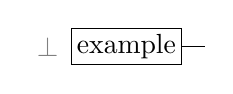
\begin{tikzpicture}
   \gen {1} {0.0} {0.0} {0} {1} {example} {1.}
\end{tikzpicture}
}
A further example of a complex, parametric generator is the macro for drawing arbitrary tape-swaps. A generator of the form $\sigma^{\oplus}_{\bullet, \bullet}$ is compiled to the macro:

\begin{lstlisting}
% posx posy n1 n2 oplusdist otimesdist tapepadding width
\swaptape 0 0 2 3 0.5 0.5 0.5 2
\end{lstlisting}
Which renders the following:

\ctbox{
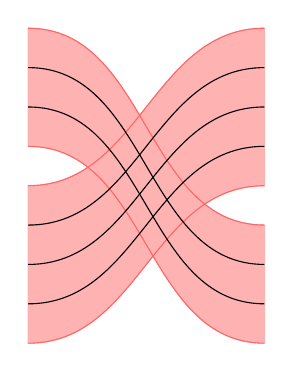
\begin{tikzpicture}
   \swaptape 0 0 2 3 {0.5} {0.5} {0.5} 3
\end{tikzpicture}
}
These basic \emph{building blocks} can then be combined and connected by the renderer to produce even very complex tape diagrams. In the following, we provide an overview of the whole drawing process.

\pagebreak
\subsubsection{The anatomy of a tape diagram}
In order to discuss how the basic building blocks can be composed, we first need to discuss what their fundamental properties are. Among these are their \emph{position}, \emph{height}, \emph{length}, and their \emph{interfaces}. Since the first three are self-explanatory, we shall focus on the fourth one. The {left} and {right interfaces} of a tape are an extension of their arity and coarity, which include information regarding the positions of the ``\emph{circuit pins}'' and the bounds of the tapes. These are defined as follows:

\begin{lstlisting}[language=ml]
 type circuit_draw_interface =
  | EmptyCircuit
  | CircuitTens of circuit_draw_interface * circuit_draw_interface
  | CircuitPin of float * float

type tape_draw_interface =
  | EmptyTape of (float * float) * (float * float)
  | TapeTens of tape_draw_interface * tape_draw_interface
  | TapeInterface of (float * float) * (float * float) * circuit_draw_interface
\end{lstlisting}
In particular, a circuit interface is essentially a list of pairs of floats, whereas a tape interface is a list of circuit interfaces together with the positions of the bounds of the tape. Note that, unlike an empty circuit, an empty tape still carries information regarding its bounds (which will not enclose a circuit).

\begin{figure}[ht]
\ctbox{
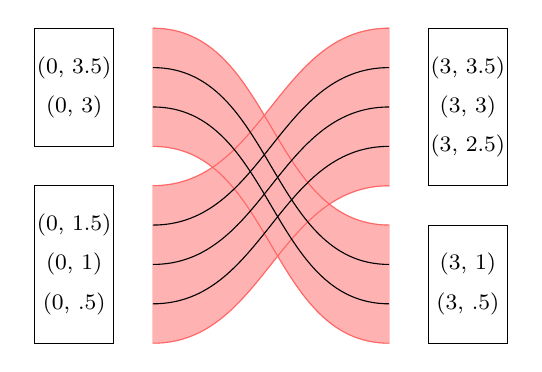
\begin{tikzpicture}
   \swaptape 0 0 2 3 {0.5} {0.5} {0.5} 3

   \draw (-.5,0) -- (-.5,2) -- (-1.5,2) -- (-1.5,0) -- cycle;

   \draw (-.5,2.5) -- (-.5,4) -- (-1.5,4) -- (-1.5,2.5) -- cycle;


   \draw (3.5,0) -- (3.5,1.5) -- (4.5,1.5) -- (4.5,0) -- cycle;

   \draw (3.5,2) -- (3.5,4) -- (4.5,4) -- (4.5,2) -- cycle;

   \node () at (-1, .5) {\footnotesize(0, .5)};
   \node () at (-1, 1) {\footnotesize(0, 1)};
   \node () at (-1, 1.5) {\footnotesize(0, 1.5)};

   \node () at (-1, 3) {\footnotesize(0, 3)};
   \node () at (-1, 3.5) {\footnotesize(0, 3.5)};

      \node () at (4, .5) {\footnotesize(3, .5)};
   \node () at (4, 1) {\footnotesize(3, 1)};

   \node () at (4, 2.5) {\footnotesize(3, 2.5)};
   \node () at (4, 3) {\footnotesize(3, 3)};
   \node () at (4, 3.5) {\footnotesize(3, 3.5)};

\end{tikzpicture}
}

\caption{A generator, together with its interfaces.}
\end{figure}
In addition to these generator-specific properties, there are also some \textbf{gloabal properties} that need to be specified. Among these are the distance between two ``lanes'' of a circuit, denoted as $d_\otimes$, the distance between two vertically stacked tapes, denoted as $d_\oplus$, and the distance the edge of a tape and the first circuit, which we will call \emph{padding distance} or $d_p$.

\begin{figure}[ht]
\ctbox{
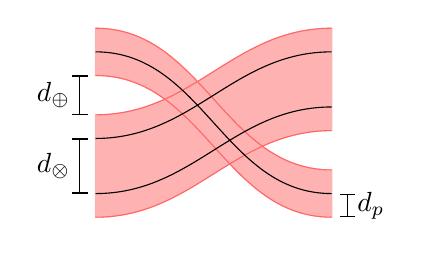
\begin{tikzpicture}
   \swaptape 0 0 1 2 {0.5} {0.7} {0.3} 3

   \draw [|-|] (3.2, 0) -- node [right] {$d_p$} (3.2, .3);
   \draw [|-|] (-.2, .3) -- node [left] {$d_\otimes$} (-.2, 1);
   \draw [|-|] (-.2, 1.3) -- node [left] {$d_\oplus$} (-.2, 1.8);


\end{tikzpicture}
}
\caption{The global properties $d_\otimes$, $d_\oplus$ and $d_p$.}
\end{figure}

We are now ready to discuss how these properties can be used to combine the generators and obtain arbitrary tape diagrams.

\subsubsection{Combining circuit generators}

There are two ways to combine the circuit generators (identity, symmetry and named generators): tensor composition and sequential composition.

\paragraph{Tensor Composition} The vertical composition is fairly straight-forward. We simply need to vertically stack the two diagrams, with a gap of length $d_\otimes$ between them:

\begin{figure}[ht]
\ctbox{
\begin{tikzpicture}
   \swap 0 0 0 1
   \id 2 0 {1.5}

\end{tikzpicture}
}
\caption{Simple example of vertical composition of circtuits.}
\end{figure}

There are some cases in which this cannot be done in the straight-forward manner: those in which the two diagrams have different lengths. In those cases we need to perform an \emph{interface alignment}, in which the right interface of the shorter circuit is extended in such a way to be aligned with the right interface of the longer circuit:

\begin{figure}[ht]
\ctbox{
\begin{tikzpicture}
   \swap 0 0 0 1
   \swap 1 1 0 1
   \id 2 0 {1.5}
   \draw [dashed, ->] (1, 1.5) -- (2, 1.5);

\end{tikzpicture}
}
\caption{Vertical composition of circuits of different length.}
\end{figure}

\paragraph{Sequential Composition} Sequential composition of circuits is simpler: we just need to horizontally stack the two circuits, making sure to place them in such a way that the interfaces match. By design of the constructors, this amounts to aligning the centers of the two circuits.

\begin{figure}[ht]
\ctbox{
\begin{tikzpicture}
   \swap 0 0 0 1
   \id 2 1 {0}
   \id 2 1 {1}
\end{tikzpicture}
}
\caption{Sequential composition of circuits.}
\end{figure}

\pagebreak

\subsubsection{Combining tape generators}
There are three ways to combine the generators to obtain non-elementary diagrams. These are tensor composition, sequential composition and the embedding of a circuit within a tape.

\paragraph{Tensor composition} Analogously to the case of circuits, we simply need to vertically stack the two tape diagrams, with a gap of length $d_\oplus$ between them.

\begin{figure}[ht]
\ctbox{
\begin{tikzpicture}
   \tape 0 0 1 1
   \id 1 0 {.5}

   \tape 0 {1.5} 1 1
   \id 2 0 {2}

\end{tikzpicture}
}
\caption{Simple example of vertical composition of tapes.}
\end{figure}
Once again, when two diagrams of different lengths are summed, we need to perform an \emph{interface alignment}, in which the right interface of the shorter tape is extended in such a way to be aligned with the right interface of the longer tape.

\begin{figure}[ht]
\ctbox{
\begin{tikzpicture}
   \tape 0 0 1 1
   \id 1 0 {.5}

   \swaptape 0 {1.5} 1 1 {0.5} {0.5} {0.5} 2

   \draw [pattern color=tapeBg, tapeBg, pattern = north east lines] (1,0) -- (1,1) -- (2,1) -- (2, 0) -- cycle;
   \draw [dashed, ->] (1, .5) -- (2, .5);
   \draw [dashed, ->, tapeBorder] (1, 0) -- (2, 0);
   \draw [dashed, ->, tapeBorder] (1, 1) -- (2, 1);

\end{tikzpicture}
}
\caption{Vertical composition of tapes with interface alignment.}
\end{figure}

\paragraph{Sequential composition} In a similar vein, when sequentially aligning two tape diagrams, we want to stack the two pictures horizontally. It might happen that two diagrams we want to horizontally compose have different heights; in these cases, we must add an \emph{adapter} between their interfaces.

\begin{figure}[ht]
\ctbox{
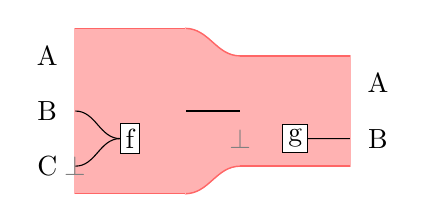
\begin{tikzpicture}[scale = .7]
\freestyletape {2.000000} {0.000000} {2.000000} {3.000000} {3.000000} {0.500000} {3.000000} {2.500000}\draw [in=180, out=0] (2.000000 , 1.500000) to (3.000000 , 1.500000);
\tape {0.000000} {0.000000} {2.000000} {3.000000}
\gen {1}{0.000000}{0.500000}{2}{0}{f}{1.000000}
\tape {3.000000} {0.500000} {2.000000} {2.000000}
\gen {2}{3.000000}{1.000000}{0}{1}{g}{1.000000}


\node () at (-0.500000, 2.500000) {A};
\node () at (-0.500000, 1.500000) {B};
\node () at (-0.500000, 0.500000) {C};
\node () at (5.500000, 2.000000) {A};
\node () at (5.500000, 1.000000) {B};
\end{tikzpicture}
}
\caption{Sequential composition of tapes with adapter.}
\end{figure}

\paragraph{Embedding of a circuit within a tape}

Embedding a circuit $c$ within a tape is also fairly straight-forward, as we simply need to build a tape of height $h_c + 2 d_p$, where $h_c$ is the height of the circuit, around the circuit itself.
Note that, by definition of the \texttt{TapeInterface} constructor, the interfaces of this new tape will be of the form:
\[ \tt TapeInterface (tape\_bot\_l, tape\_top\_l, left\_interface(c)) \]
\[ \tt TapeInterface (tape\_bot\_r, tape\_top\_r, right\_interface(c)) \]



\begin{figure}[ht]
\ctbox{
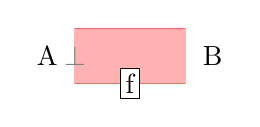
\begin{tikzpicture}[scale = .7]
\tape {0.000000} {0.000000} {2.000000} {1.000000}
\gen {1}{0.000000}{0.500000}{0}{0}{f}{1.000000}

\node () at (-0.500000, 0.500000) {A};
\node () at (2.500000, 0.500000) {B};
\end{tikzpicture}
}
\caption{Generator embedded within a tape.}
\end{figure}

\subsubsection{Examples of complex circuits}

\begin{figure}[ht]
\ctbox{
\begin{tikzpicture}[scale = .7]
\freestyletape {6.000000} {2.500000} {6.000000} {5.500000} {7.000000} {2.500000} {7.000000} {5.500000}\draw [in=180, out=0] (6.000000 , 5.000000) to (7.000000 , 5.000000);
\draw [in=180, out=0] (6.000000 , 4.000000) to (7.000000 , 4.000000);
\draw [in=180, out=0] (6.000000 , 3.000000) to (7.000000 , 3.000000);
\freestyletape {6.000000} {0.000000} {6.000000} {2.000000} {7.000000} {0.000000} {7.000000} {2.000000}\draw [in=180, out=0] (6.000000 , 1.500000) to (7.000000 , 1.500000);
\draw [in=180, out=0] (6.000000 , 0.500000) to (7.000000 , 0.500000);
\tape {0.000000} {2.500000} {6.000000} {3.000000}
\gen {1}{0.000000}{3.500000}{0}{1}{f}{1.000000}
\id{3}{2.000000}{4.500000}
\gen {2}{2.000000}{3.500000}{0}{0}{g}{1.000000}
% adjusting misaligned tensors:
\draw [in=180, out=0] (3.000000 , 4.500000) to (4.000000 , 4.500000);
\draw [in=180, out=0] (4.000000 , 3.500000) to (4.000000 , 3.500000);
% composing interfaces:
\draw [in=180, out=0] (2.000000 , 4.500000) to (2.000000 , 4.500000);
\draw [in=180, out=0] (2.000000 , 3.500000) to (2.000000 , 3.500000);
\gen {3}{4.000000}{3.000000}{1}{2}{h}{1.000000}
% composing interfaces:
\draw [in=180, out=0] (4.000000 , 4.500000) to (4.000000 , 4.500000);
\draw [in=180, out=0] (4.000000 , 3.500000) to (4.000000 , 3.500000);
\tape {0.000000} {0.000000} {1.000000} {2.000000}
\id{2}{0.000000}{1.500000}
\id{1}{0.000000}{0.500000}
% adjusting misaligned tensors:
\draw [in=180, out=0] (1.000000 , 1.500000) to (1.000000 , 1.500000);
\draw [in=180, out=0] (1.000000 , 0.500000) to (1.000000 , 0.500000);
\freestyletape {6.000000} {2.500000} {6.000000} {5.500000} {6.000000} {2.500000} {6.000000} {5.500000}\draw [in=180, out=0] (6.000000 , 5.000000) to (6.000000 , 5.000000);
\draw [in=180, out=0] (6.000000 , 4.000000) to (6.000000 , 4.000000);
\draw [in=180, out=0] (6.000000 , 3.000000) to (6.000000 , 3.000000);
\freestyletape {1.000000} {0.000000} {1.000000} {2.000000} {6.000000} {0.000000} {6.000000} {2.000000}\draw [in=180, out=0] (1.000000 , 1.500000) to (6.000000 , 1.500000);
\draw [in=180, out=0] (1.000000 , 0.500000) to (6.000000 , 0.500000);
\swaptape {7.000000} {0.000000} {3} {2} {0.500000} {1.000000} {0.500000} {2.000000}
\node () at (-0.500000, 4.000000) {A};
\node () at (-0.500000, 1.500000) {A};
\node () at (-0.500000, 0.500000) {B};
\node () at (9.500000, 5.000000) {A};
\node () at (9.500000, 4.000000) {B};
\node () at (9.500000, 2.500000) {D};
\node () at (9.500000, 1.500000) {E};
\node () at (9.500000, 0.500000) {F};
\end{tikzpicture}
}
\caption{$\tt{(\underline{\overline{gen(f, A, AB) ; (id(A) \otimes gen(g, B, C)) ; gen(h, AC, DEF)}} \oplus
id(A\otimes B));
\sigma^{\oplus}_{DEF, AB}}$}
\end{figure}


\end{document}
